%
% problemstellung.tex 
%
% 
%
% !TEX root = ../../buch.tex
% !TEX encoding = UTF-8
%
\section{Aufgabenstellung\label{antennen:problemstellung}}
 Es soll eine Antennenform designed werden, welche in einem Gerät mit der Form 
 eines Prismas mit Deckfläche eines gleichseitigen Dreiecks Platz findet. Dies bedeutet, dass 
 die Form das Mass eines gleichseitigen Dreiecks nicht überschreiten darf.
 
\subsection{Geometrie\label{antennen:Geom}}
Das Ziel ist nun, den Wirkungsgrad durch Formoptimierung zu erhöhen. Es soll eine optimale Form
gefunden werden, welche vorherige Einschränkungen einhält.
Die Faktoren $k\textsubscript{1}$ und $k\textsubscript{2}$ sind Konstanten. 
Dies bedeutet, dass für eine Erhöhung des Wirkungsgrads \eqref{antennen:Wirkungsgradeingesetzt} nur die Länge 
$l$ und die Fläche $A$ relevant und veränderbar sind. In einem nächsten Schritt wird das Verhältnis
\begin{equation}
	\frac{l}{A^2} \rightarrow \frac{l}{A}
	\label{antennen:Verhältnis}
\end{equation}
verkleinert. 
Der Pfeil in \eqref{antennen:Verhältnis} weist darauf hin, dass eine Minimierung des Verhältnisses zwischen Länge und Fläche im Quadrat auch eine Minimierung des Verhältnisses zwischen Länge und Fläche zur Folge hat. Dieses Vorgehen darf in einem Minimalproblem nur verwendet werden, wenn die Parameter $l$ und $A$ unabhängig voneinander sind. Somit kann dieser Ausdruck 
für den weiteren Verlauf vereinfacht werden. Diese vereinfachte Formel kann nun auf eine implizite 
Funktion angewendet werden. Die Funktion gibt dann Auskunft über die aufgespannte Fläche und 
dem Umfang. Somit kann das Verhältnis \eqref{antennen:Verhältnis} gezielt optimiert werden. 

In den Ecken wird für einen minimale Flächenvergrösserung viel Länge gebraucht.
Eine erste, nicht mathematische Idee besteht darin, die Ecken abzurunden. Dies ist in Abbildung
\ref{antennen:tikabgerundet} zu sehen. 

Eine weitere Idee wäre es, die Ecken wie in der Abbildung \ref{antennen:tikabgeflacht} abzuflachen. Bei
beiden Ideen muss noch bestimmt werden, wo genau die Anpassung der Eckstücke gemacht werden muss. Dies ist in den Abbildungen 
\ref{antennen:tikabgeflacht_kleiner} und \ref{antennen:tikabgerundet_kleiner} veranschaulicht.

\begin{figure}
	\centering
	\begin{minipage}[t]{0.45\textwidth}
		\centering
		\begin{tikzpicture}

			\def\sidelength{3.14}
			
			\pgfmathsetmacro{\triangleheight}{sqrt(3)/2*\sidelength}

			\draw[fill=white] (0,0) -- (\sidelength,0) -- (0.5*\sidelength, \triangleheight) -- cycle;
			
			\draw[red, line width=0.3mm, rounded corners=0.5cm] (0,0) -- (\sidelength,0) -- (0.5*\sidelength, \triangleheight) -- cycle;
			
			\draw[->,{line width=0.5pt},>={Stealth[scale=0.62]}] (-0.35,0) -- (3.7,0) node[above 	left] {$x$};
			\draw[->,{line width=0.5pt},>={Stealth[scale=0.62]}] (0,-0.785) -- (0,3.14) node[below right] {$y$};
			
			\foreach \x\xlabel in {1.5708/$\frac{\pi}{2}$, 3.14159/$\pi$}
			\draw (\x,2pt) -- (\x,-2pt) node[below] {\xlabel};
		\end{tikzpicture}
		\caption{Antenne mit abgerundeten Ecken.}
		\label{antennen:tikabgerundet}
	\end{minipage}
	\hfill
	\begin{minipage}[t]{0.45\textwidth}
		\centering
		\begin{tikzpicture}
			\def\sidelength{3.14}
			
			\pgfmathsetmacro{\triangleheight}{sqrt(3)/2*\sidelength}

			\draw[fill=white] (0,0) -- (\sidelength,0) -- (0.5*\sidelength, \triangleheight) -- cycle;
			
			\draw[red, line width=0.3mm] 
			(0.5,0) -- (0.25,1.73/2*0.5) -- (0.5*\sidelength-0.25, \triangleheight-1.73/2*0.5) -- 
			(0.5*\sidelength+0.25, \triangleheight-1.73/2*0.5) -- (\sidelength-0.25,1.73/2*0.5) -- (\sidelength-0.5,0) -- cycle;
			
			\draw[->,{line width=0.5pt},>={Stealth[scale=0.62]}] (-0.35,0) -- (3.7,0) node[above left] {$x$};
			\draw[->,{line width=0.5pt},>={Stealth[scale=0.62]}] (0,-0.785) -- (0,3.14) node[below right] {$y$};
			
			\foreach \x\xlabel in {1.5708/$\frac{\pi}{2}$, 3.14159/$\pi$}
			\draw (\x,2pt) -- (\x,-2pt) node[below] {\xlabel};
		\end{tikzpicture}
		\caption{Antennenform mit abgeflachten Ecken.}
		\label{antennen:tikabgeflacht}
	\end{minipage}

\end{figure}

\begin{figure}
	\centering
	\begin{minipage}[t]{0.45\textwidth}
		\centering
		\begin{tikzpicture}
			\definecolor{clrGreen}{RGB}{0, 117, 18}

			\def\sidelength{3.14}
			
			\pgfmathsetmacro{\triangleheight}{sqrt(3)/2*\sidelength}

			\draw[fill=white] (0,0) -- (\sidelength,0) -- (0.5*\sidelength, \triangleheight) -- cycle;
			
			\draw[red, line width=0.3mm,] (0.5,0) -- (0.25,1.73 /2*0.5) -- (0.5*\sidelength-0.25, \triangleheight-1.73/2*0.5) -- (0.5*\sidelength+0.25, \triangleheight-1.73/2*0.5)--(\sidelength-0.25,1.73/2*0.5) -- (\sidelength-0.5,0) -- cycle;
			
			\draw[clrGreen, line width=0.3mm,] (1,0) -- (0.5,1.73 /2*1) -- (0.5*\sidelength-0.5, \triangleheight-1.73/2*1) -- (0.5*\sidelength+0.5, \triangleheight-1.73/2*1)--(\sidelength-0.5,1.73/2*1) -- (\sidelength-1,0) -- cycle;
			
			\draw[blue, line width=0.3mm,] (1.5,0) -- (0.75,1.73 /2*1.5) -- (0.5*\sidelength-0.75, \triangleheight-1.73/2*1.5) -- (0.5*\sidelength+0.75, \triangleheight-1.73/2*1.5)--(\sidelength-0.75,1.73/2*1.5) -- (\sidelength-1.5,0) -- cycle;
			
			\draw[->,{line width=0.5pt},>={Stealth[scale=0.62]}] (-0.35,0) -- (3.7,0) node[above left] {$x$};
			\draw[->,{line width=0.5pt},>={Stealth[scale=0.62]}] (0,-0.785) -- (0,3.14) node[below right] {$y$};
			
			\foreach \x/\xlabel in {1.5708/$\frac{\pi}{2}$, 3.14159/$\pi$}
			\draw (\x,2pt) -- (\x,-2pt) node[below] {\xlabel};
		\end{tikzpicture}
		\caption{Antennenform mit variablen abgeflachten Ecken.}
		\label{antennen:tikabgeflacht_kleiner}
	\end{minipage}
	\hfill
	\begin{minipage}[t]{0.45\textwidth}
		\centering
		\begin{tikzpicture}
			\definecolor{clrGreen}{RGB}{0, 117, 18}

			\def\sidelength{3.14}
			
			\pgfmathsetmacro{\triangleheight}{sqrt(3)/2*\sidelength}

			\draw[fill=white] (0,0) -- (\sidelength,0) -- (0.5*\sidelength, \triangleheight) -- cycle;
			
			\draw[red, line width=0.3mm, rounded corners=0.5cm] (0,0) -- (\sidelength,0) -- (0.5*\sidelength, \triangleheight) -- cycle;
			
			\draw[clrGreen, line width=0.3mm, rounded corners=1cm] (0,0) -- (\sidelength,0) -- (0.5*\sidelength, \triangleheight) -- cycle;
			
			\draw[blue, line width=0.3mm, rounded corners=1.5cm] (0,0) -- (\sidelength,0) -- (0.5*\sidelength, \triangleheight) -- cycle;
			
			\draw[->,{line width=0.5pt},>={Stealth[scale=0.62]}] (-0.35,0) -- (3.7,0) node[above left] {$x$};
			\draw[->,{line width=0.5pt},>={Stealth[scale=0.62]}] (0,-0.785) -- (0,3.14) node[below right] {$y$};
			
			\foreach \x/\xlabel in {1.5708/$\frac{\pi}{2}$, 3.14159/$\pi$}
			\draw (\x,2pt) -- (\x,-2pt) node[below] {\xlabel};
		\end{tikzpicture}
		\caption{Antennenform mit variablen abgerundeten Ecken.}
		\label{antennen:tikabgerundet_kleiner}
	\end{minipage}%
\end{figure}
Eine Eigenschaft, die das Problem vereinfacht, ist die Symmetrie des Dreiecks. 
\index{Symmetrie}%
Das Gesamtproblem kann vereinfacht werden indem nur eine Ecke betrachtet wird. 
Wie in der Abbildung \ref{antennen:tikzAntenneSymmetrie} dargestellt, sind die drei Eckfunktionen äquivalent. Die drei 
gestrichelten Geraden spannen ein weiteres gleichseitiges Dreieck auf. Dieses kann jedoch vernachlässigt werden, da es für alle gesuchten Funktionen $f(x,y)$ 
gleich bleibt. Somit ist das implizite Problem $f(x,y)$ zur expliziten Funktion $f(x)$ 
geworden, die wesentlich leichter zu optimieren ist.

\begin{figure}
	\centering
	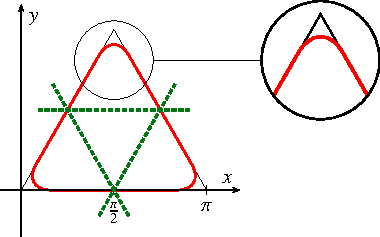
\includegraphics{papers/antennen/images/SymmetrieDreieck.pdf}
	\caption{Symmetrie der Antenne.}
	\label{antennen:tikzAntenneSymmetrie}
\end{figure}






